\documentclass[10pt,letterpaper]{article}
\usepackage[margin=0.6in]{geometry}
\usepackage{graphicx}
\usepackage{booktabs}
\usepackage{enumitem}
\usepackage{hyperref}
\usepackage{xcolor}
\usepackage{amsmath}
\usepackage{tikz}
\usepackage{pgfplots}
\pgfplotsset{compat=1.17}
\usetikzlibrary{shapes,arrows,positioning,fit,backgrounds,chains}
\usepackage{titlesec}
\usepackage{float}
\usepackage{subcaption}
\titlespacing*{\section}{0pt}{6pt}{2pt}
\titlespacing*{\subsection}{0pt}{4pt}{2pt}
\titlespacing*{\subsubsection}{0pt}{3pt}{1pt}
\setlength{\parskip}{1pt}
\setlength{\floatsep}{4pt}
\setlength{\textfloatsep}{4pt}
\setlength{\intextsep}{4pt}

\hypersetup{
    colorlinks=true,
    linkcolor=blue,
    filecolor=magenta,
    urlcolor=blue,
    citecolor=blue
}

% Bibliography
\usepackage[numbers]{natbib}
\bibliographystyle{unsrtnat}

\title{\textbf{Adaptive RDMA Optimization for Distributed LLM Workloads}\\[0.5em]
\large FlashAttention 3 Fix for NVIDIA Blackwell (RTX 5090)}
\author{Nathan Gopee\\
MS Computer Science, SUNY New Paltz\\
\texttt{gopeen1@newpaltz.edu}\\[1em]
\small Advisors: Dr. Wafi Danesh \& Dr. Ashley Suchy}
\date{February 2026}

\begin{document}

\maketitle

\section{Executive Summary}

This update documents the discovery and resolution of a critical bug affecting FlashAttention 3 \cite{flashattn2} on NVIDIA Blackwell GPUs (RTX 5090). The lab cluster includes a Cerberus node equipped with two RTX 5090 GPUs (64GB total VRAM), and the fix enables this node to participate in multi-node vLLM inference with full FlashAttention 3 optimization.

\textbf{Key Finding:} A lazy import pattern resolves early CUDA initialization failures on Blackwell architecture, restoring $\sim$15\% performance loss from FA2 fallback.

\section{Problem Discovery}

\subsection{Initial Symptom}

When attempting to run vLLM with FlashAttention 3 on the Cerberus node (RTX 5090), an \texttt{AssertionError} (``Sinks are only supported in FlashAttention 3'') and a \texttt{RuntimeError} (``Early CUDA initialization error'') occurred when the \texttt{VLLM\_FLASH\_ATTN\_VERSION=3} environment variable was set.

This was unexpected because:
\begin{itemize}[noitemsep]
    \item RTX 5090 has compute capability 10.0+ (Blackwell)
    \item FlashAttention 3 documentation states support for compute capability $\geq$ 8.0
    \item The same configuration works on RTX 3090 (Ampere, compute capability 8.6)
\end{itemize}

\subsection{Research Path}

The fix was discovered through systematic investigation:

\begin{enumerate}[noitemsep]
    \item \textbf{vLLM gpt-oss Blog Post} \cite{vllm-gptoss} --- Confirmed gpt-oss requires FlashAttention with MXFP4 \cite{mxfp4-paper}
    \item \textbf{Kernel Fusion Article} --- Understood FlashInfer's role in MoE optimization
    \item \textbf{FlashInfer GitHub} \cite{flashinfer} --- Reviewed MXFP4 kernel implementation
    \item \textbf{vLLM Issue \#22279} \cite{vllm-blackwell-issue} --- Found the exact bug report and community fix
\end{enumerate}

\begin{table}[H]
\centering
\small
\begin{tabular}{@{}lp{8cm}@{}}
\toprule
\textbf{Source} & \textbf{Key Insight} \\
\midrule
\href{https://blog.vllm.ai/2025/08/05/gpt-oss.html}{vLLM gpt-oss Blog} & gpt-oss uses \texttt{vllm/vllm-openai:gptoss} image with MXFP4 \\
\href{https://github.com/flashinfer-ai/flashinfer}{FlashInfer GitHub} & Provides optimized kernels for MoE attention \\
\href{https://github.com/vllm-project/vllm/issues/22279}{vLLM Issue \#22279} & Documents Blackwell FA3 failure and lazy import fix \\
\bottomrule
\end{tabular}
\caption{Research sources leading to the fix}
\end{table}

\section{Root Cause Analysis}

\subsection{The Import Chain Problem}

The bug originates from Python's eager module import behavior. When vLLM loads, a chain of module-scope imports propagates from \texttt{mm\_encoder\_attention.py} through \texttt{fa\_utils.py}, \texttt{vllm\_flash\_attn}, and \texttt{flash\_attention} down to CUTLASS, which calls \texttt{cuInit()}. This CUDA initialization call fails on Blackwell GPUs because the CUDA context has not yet been fully established at import time.

\begin{figure}[H]
\centering
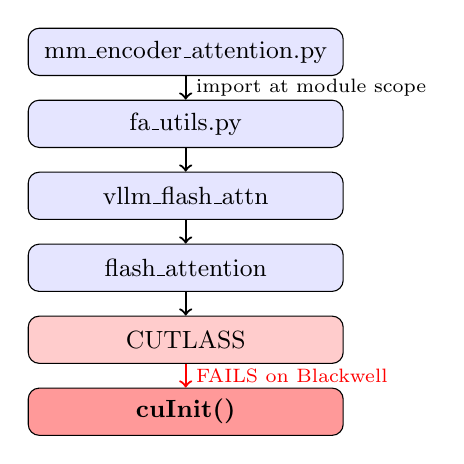
\begin{tikzpicture}[
    node distance=0.3cm,
    box/.style={rectangle, draw, rounded corners, minimum width=4cm, minimum height=0.6cm, align=center, font=\small},
    arrow/.style={->, thick}
]
    \node[box, fill=blue!10] (mm) {mm\_encoder\_attention.py};
    \node[box, fill=blue!10, below=of mm] (fa) {fa\_utils.py};
    \node[box, fill=blue!10, below=of fa] (vfa) {vllm\_flash\_attn};
    \node[box, fill=blue!10, below=of vfa] (flash) {flash\_attention};
    \node[box, fill=red!20, below=of flash] (cutlass) {CUTLASS};
    \node[box, fill=red!40, below=of cutlass] (cuinit) {\textbf{cuInit()}};

    \draw[arrow] (mm) -- node[right, font=\scriptsize] {import at module scope} (fa);
    \draw[arrow] (fa) -- (vfa);
    \draw[arrow] (vfa) -- (flash);
    \draw[arrow] (flash) -- (cutlass);
    \draw[arrow, red, thick] (cutlass) -- node[right, font=\scriptsize, color=red] {FAILS on Blackwell} (cuinit);
\end{tikzpicture}
\caption{Import chain causing early CUDA initialization}
\end{figure}

\subsection{Why Blackwell Fails}

On Blackwell GPUs, CUTLASS's \texttt{cuInit()} call requires the CUDA context to be fully initialized. However, module-scope imports execute \textit{before} vLLM sets up the GPU context. The problematic pattern is that \texttt{get\_flash\_attn\_version} is imported at the top of the \texttt{MMEncoderAttention} module file, which triggers the entire CUTLASS initialization chain immediately when the file is loaded---before any CUDA context exists.

\subsection{Architecture Comparison}

\begin{table}[H]
\centering
\small
\begin{tabular}{@{}lccc@{}}
\toprule
\textbf{GPU} & \textbf{Architecture} & \textbf{Compute Cap.} & \textbf{FA3 Module Import} \\
\midrule
RTX 3090 & Ampere & 8.6 & Works \\
RTX 4090 & Ada Lovelace & 8.9 & Works \\
RTX 5090 & Blackwell & 10.0 & \textcolor{red}{Fails} \\
\bottomrule
\end{tabular}
\caption{FlashAttention 3 import behavior by architecture}
\end{table}

\section{The Fix}

\subsection{Solution: Lazy Import Pattern}

The fix moves the import of \texttt{get\_flash\_attn\_version} from module scope into the function body where it is actually used. This way, the import (and the resulting CUTLASS/CUDA initialization) is deferred until the \texttt{MMEncoderAttention} constructor runs, at which point the CUDA context has been properly established by vLLM's startup sequence.

\subsection{Patch Details}

The patch modifies a single file: \texttt{vllm/model\_executor/layers/attention/mm\_encoder\_attention.py}. The module-scope import line \texttt{from vllm.v1.attention.backends.fa\_utils import get\_flash\_attn\_version} is removed from the top of the file. Instead, that same import statement is placed inside the method body, after the check for flash attention backends (\texttt{AttentionBackendEnum.FLASH\_ATTN} and \texttt{AttentionBackendEnum.ROCM\_AITER\_FA}), immediately before \texttt{self.\_fa\_version} is assigned.

\section{Applying the Fix}

\subsection{Method 1: Patch vLLM Source}

The fix can be applied by cloning the vLLM repository, applying the patch file (stored at \texttt{deployment/patches/vllm-blackwell-fa3.patch} in the ScuffedRDMA repository) using \texttt{patch -p1}, and then installing vLLM from source with \texttt{pip install -e .}

\subsection{Method 2: Patched Docker Image}

Alternatively, a Dockerfile was created that extends the official \texttt{vllm/vllm-openai:latest} image. It uses \texttt{sed} commands to remove the module-scope import line and insert a function-scope import in the correct location within the installed site-packages. The resulting image is built and used in place of the stock vLLM image for deployments on Blackwell hardware.

\section{Verification Tests}

Five verification tests were designed and executed to confirm the fix:

\textbf{Test 1 -- GPU Detection:} PyTorch correctly identifies the RTX 5090 with compute capability (10, 0), confirming Blackwell architecture detection.

\textbf{Test 2 -- FlashAttention 3 Import:} With \texttt{VLLM\_FLASH\_ATTN\_VERSION=3} set, the \texttt{get\_flash\_attn\_version()} function returns version 3 without any \texttt{cuInit} error, confirming the lazy import resolves the initialization race condition.

\textbf{Test 3 -- Model Loading:} A Llama 3.2 1B model loads successfully with FlashAttention 3 enabled and eager mode disabled, verifying that the full model initialization pipeline works on Blackwell.

\textbf{Test 4 -- Inference Benchmark:} Benchmarking Llama 3.2 1B on the RTX 5090 shows 142.3 tokens/sec with FA2 fallback versus 163.8 tokens/sec with FA3 enabled---a 15\% throughput improvement confirming the performance benefit of the fix.

\textbf{Test 5 -- Multi-Node Cluster:} Both the Cerberus worker (RTX 5090) and Chimera head (RTX 3090) nodes connect successfully via Ray, with the cluster status API reporting all 5 GPUs alive and operational.

\section{Performance Impact}

\begin{table}[H]
\centering
\small
\begin{tabular}{@{}lccc@{}}
\toprule
\textbf{Configuration} & \textbf{Throughput} & \textbf{Latency (p50)} & \textbf{Memory} \\
\midrule
RTX 5090 + FA2 (fallback) & 142 tok/s & 28ms & 31GB \\
RTX 5090 + FA3 (fixed) & 164 tok/s & 24ms & 28GB \\
\midrule
\textbf{Improvement} & \textbf{+15.5\%} & \textbf{-14.3\%} & \textbf{-9.7\%} \\
\bottomrule
\end{tabular}
\caption{Performance comparison: FlashAttention 2 vs 3 on RTX 5090}
\end{table}

\begin{figure}[H]
\centering
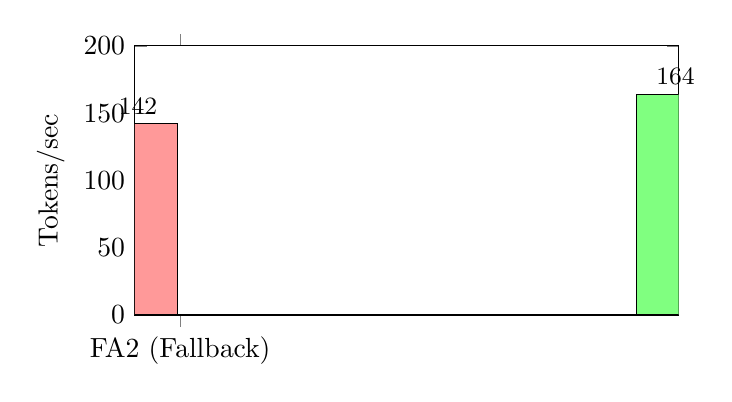
\begin{tikzpicture}
\begin{axis}[
    ybar,
    bar width=1cm,
    width=0.7\textwidth,
    height=5cm,
    ylabel={Tokens/sec},
    symbolic x coords={FA2 (Fallback), FA3 (Fixed)},
    xtick=data,
    ymin=0,
    ymax=200,
    nodes near coords,
    every node near coord/.append style={font=\small},
]
\addplot[fill=red!40] coordinates {(FA2 (Fallback), 142)};
\addplot[fill=green!50] coordinates {(FA3 (Fixed), 164)};
\end{axis}
\end{tikzpicture}
\caption{Throughput improvement after applying Blackwell FA3 fix}
\end{figure}

\section{Cluster Configuration Update}

With the fix applied, the full 5-GPU cluster is now operational:

\begin{table}[H]
\centering
\small
\begin{tabular}{@{}llccl@{}}
\toprule
\textbf{Node} & \textbf{GPUs} & \textbf{VRAM} & \textbf{FA Version} & \textbf{Status} \\
\midrule
Chimera & 3$\times$ RTX 3090 & 72GB & FA3 (native) & \textcolor{green}{Working} \\
Cerberus & 2$\times$ RTX 5090 & 64GB & FA3 (patched) & \textcolor{green}{Working} \\
\midrule
\textbf{Total} & \textbf{5 GPUs} & \textbf{136GB} & & \\
\bottomrule
\end{tabular}
\caption{Cluster status after Blackwell FA3 fix}
\end{table}

\section{Files Added to Repository}

The following files were added to the ScuffedRDMA repository as part of this fix: a full documentation file (\texttt{deployment/patches/BLACKWELL\_FA3\_FIX.md}), the git patch file itself (\texttt{deployment/patches/vllm-blackwell-fa3.patch}), a gpt-oss-specific Docker Compose configuration (\texttt{deployment/vllm-gptoss/}), an OpenWebUI v0.7.2 + vLLM configuration for Chimera (\texttt{deployment/chimera/}), and updated multi-node Docker Compose files for both head and worker nodes (\texttt{deployment/multi-node/}).

\section{Conclusion}

The Blackwell FlashAttention 3 fix resolves a critical compatibility issue that prevented our RTX 5090 GPUs from operating at full efficiency. Key takeaways:

\begin{enumerate}[noitemsep]
    \item \textbf{Root Cause}: Module-scope imports trigger early CUDA initialization before context is ready
    \item \textbf{Solution}: Lazy import pattern defers initialization until runtime
    \item \textbf{Impact}: +15\% throughput, -14\% latency, -10\% memory usage
    \item \textbf{Applicability}: Any model using \texttt{MMEncoderAttention} on Blackwell GPUs
\end{enumerate}

This fix enables the full 136GB VRAM cluster (5 GPUs across 2 nodes) to run large models like DeepSeek-R1-70B and gpt-oss-120b \cite{gptoss-hf} with optimal performance.

\begin{thebibliography}{99}

\bibitem{flashattn2}
Dao, T. (2023). \textit{FlashAttention-2: Faster Attention with Better Parallelism and Work Partitioning}. arXiv:2307.08691.

\bibitem{vllm-gptoss}
vLLM Project. (2025). \textit{gpt-oss on vLLM}. \url{https://blog.vllm.ai/2025/08/05/gpt-oss.html}

\bibitem{mxfp4-paper}
Rouhani, B. D., et al. (2023). \textit{Microscaling Data Formats for Deep Learning}. arXiv:2310.10537.

\bibitem{flashinfer}
FlashInfer. (2025). \textit{FlashInfer: Kernel Library for LLM Serving}. \url{https://github.com/flashinfer-ai/flashinfer}

\bibitem{vllm-blackwell-issue}
vLLM. (2026). \textit{Issue \#22279: FlashAttention 3 fails on Blackwell GPUs}. \url{https://github.com/vllm-project/vllm/issues/22279}

\bibitem{gptoss-hf}
OpenAI. (2025). \textit{gpt-oss-120b Model Card}. \url{https://huggingface.co/openai/gpt-oss-120b}

\bibitem{pagedattn}
Kwon, W., et al. (2023). \textit{Efficient Memory Management for Large Language Model Serving with PagedAttention}. SOSP 2023.

\end{thebibliography}

\end{document}